\documentclass[en, listings]{labreport}
\subject{System Software Fundamentals}
\titleparts{Lab Work \#6 (4)}{TCP/IP Communication}
\students{Timothy Labushev}

\usepackage{multicol}

\begin{document}

\maketitlepage

\section*{Assignment}

\subsection*{Part I}

Implement client-server communication over TCP/IP in C and Perl.\\

The client should:
\begin{enumerate}
\item Accept \textit{host name} and \textit{directory paths} as command line arguments;
\item Establish a TCP/IP connection and request file listings for the specified directories;
\item Output the listing to \texttt{stdout}.
\end{enumerate}

The server should:
\begin{enumerate}
\item Use a text protocol;
\item Handle multiple simultaneous connections;
\item Create a new thread (using \texttt{pthread}s) for each connection.
\end{enumerate}

In addition to this, the following diagrams should be provided:
\begin{itemize}
\item a BPMN diagram;
\item UML sequence, class, activity, use case, deployment, state, and component diagrams,
  written using the PlantUML notation.
\end{itemize}

\section*{Code Listing}

\verb|.c|, \verb|.pl|, and \verb|.plantuml| files are available at
\begin{verbatim}
https://github.com/timlathy/itmo-third-year/tree/master/
System-Programming-Fundamentals-5th-Term/Lab6-TCP
\end{verbatim}

\section*{Communication Protocol}

The following text protocol was implemented:

\begin{verbatim}
<request> ::= <path> { <path> } CR LF
<path> ::= <non-empty string not including NUL or CR or LF> CR LF
\end{verbatim}

\newpage

\section*{Example Telnet Interaction}

\begin{verbatim}
Trying 127.0.0.1...
Connected to 127.0.0.1.
Escape character is '^]'.
test
test-protected
.

Contents of test:
.
h
..
abc

Failed to open test-protected: Permission denied

Contents of .:
test-protected
.
test
..


Connection closed by foreign host.
\end{verbatim}

\section*{Diagrams}

\subsection*{BPMN}
\noindent
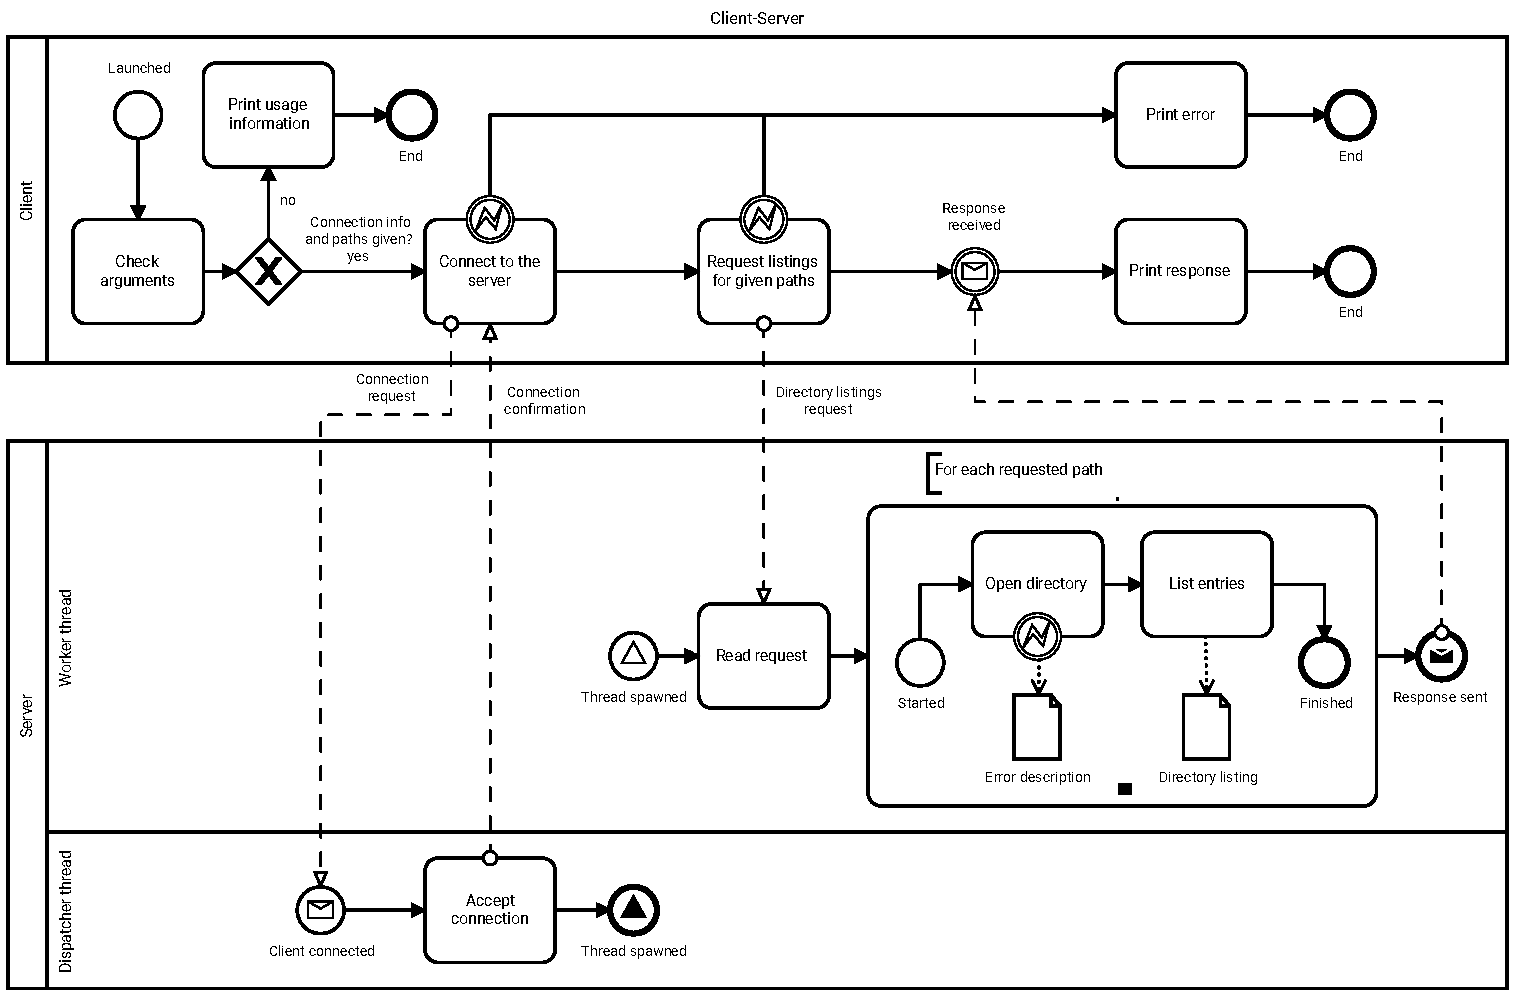
\includegraphics[width=1.05\textwidth]{diagrams/bpmn}

\subsection*{UML Use Case}
\noindent
\includegraphics[width=0.45\textwidth]{diagrams/usecase}

\subsection*{UML Sequence}
\noindent
\includegraphics[width=0.8\textwidth]{diagrams/sequence}

\subsection*{UML Activity}
\noindent
\includegraphics[width=0.9\textwidth]{diagrams/activity}

\begin{multicols}{2}

\subsection*{UML State}
\noindent
\includegraphics[width=0.45\textwidth]{diagrams/state}

\subsection*{UML Component}
\noindent
\includegraphics[width=0.5\textwidth]{diagrams/component}

\end{multicols}

\subsection*{UML Deployment}
\noindent
\includegraphics[width=0.8\textwidth]{diagrams/deployment}

\end{document}
